\subsection{Qualità di processo - Fornitura}

\vspace{0.3cm}

\subsubsection{M1PMS - Percentuale di Metriche Soddisfatte}
\begin{figure}[H]
    \centering
    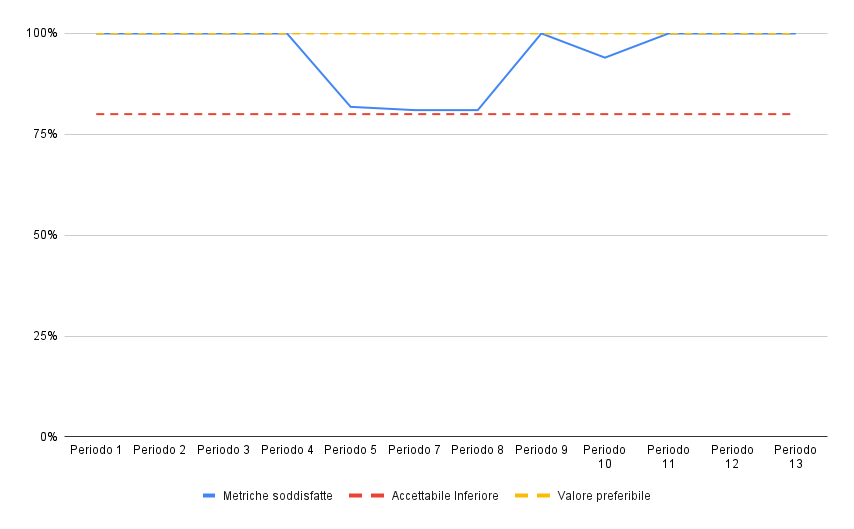
\includegraphics[width=1\textwidth]{../Images/PianoDiQualifica/M1PMS.png}
    \caption{Proiezione della percentuale di metriche soddisfatte nei vari periodi di progetto.}
    \label{fig:1}
\end{figure}

\vspace{0.2cm}

\textbf{RTB}: nel corso dei primi periodi, è evidente l'adozione di tutte le metriche di qualità; tuttavia, è solamente nell'ultimo periodo che si osserva il superamento dei valori di accettazione per due metriche, M2EAC e M4BV, fenomeno attribuibile al periodo di esami universitari.

\vspace{0.2cm}

\textbf{PB}: Il grafico evidenzia un’adozione efficace delle metriche di qualità. Nonostante ci siano stati periodi con percentuali inferiori, queste rimangono sempre all’interno dei range di accettazione. La diminuzione osservata è attribuibile alle metriche dedicate ai test data e al mancato raggiungimento dei valori di accettazione per alcune metriche, a causa della limitata esperienza del gruppo in questo specifico ambito. Durante il decimo periodo, si è verificato un superamento dei valori di accettazione per la metrica M24DE, causato dall’introduzione di uno strumento per la valutazione della qualità del codice. Questi problemi sono stati prontamente risolti e, nel periodo immediatamente successivo, la percentuale di metriche soddisfatte è ritornata ai valori ottimali.

\subsubsection{M2EAC - Estimed at Completion}

\vspace{0.3cm}

\begin{figure}[H]
    \centering
    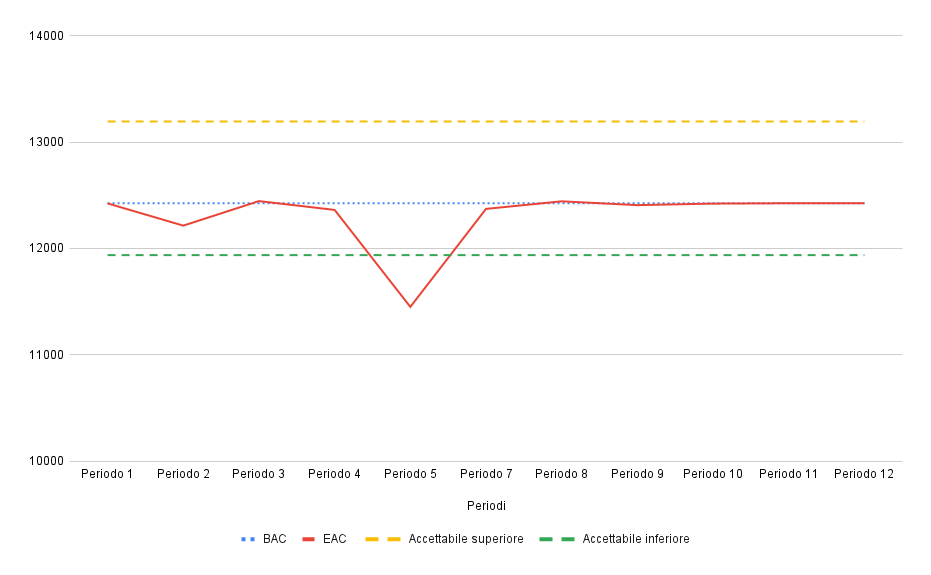
\includegraphics[width=1\textwidth]{../Images/PianoDiQualifica/M2EAC.png}
    \caption{Proiezione della stima del costo totale nei vari periodi di progetto.}
    \label{fig:2}
\end{figure}

\vspace{0.2cm}

\textbf{RTB}: si nota come nei primi periodi la stima del costo totale sia in linea con il budget inzialmente preventivato.

Tuttavia al quinto periodo, periodo di sessione degli esami, il costo totale è di molto inferiore al budget preventivato.

Questo è dovuto al fatto che in quel periodo c'è stato un calo di \textit{attività}\textsubscript{\textit{G}}, in quanto i membri del gruppo erano impegnati con gli esami universitari. Le \textit{attività}\textsubscript{\textit{G}} però rimanenti sono state completate con un costo inferiore a quello preventivato e questo ha portato ad una riduzione del costo totale.\\
\vspace{0.2cm}

\textbf{PB}: si nota come, nei restanti dei periodi,nonostante una diminuzione registrata nel quinto periodo, la stima del costo totale è rientrata nei limiti di accettazione. Inoltre, tale stima è rimasta in stretta aderenza al budget preventivato. Questo fenomeno indica un’efficace gestione dei costi.


\subsubsection{M7EV- Earned Value + M8PV - Planned Value} 

\vspace{0.3cm}

\begin{figure}[H]
    \centering
    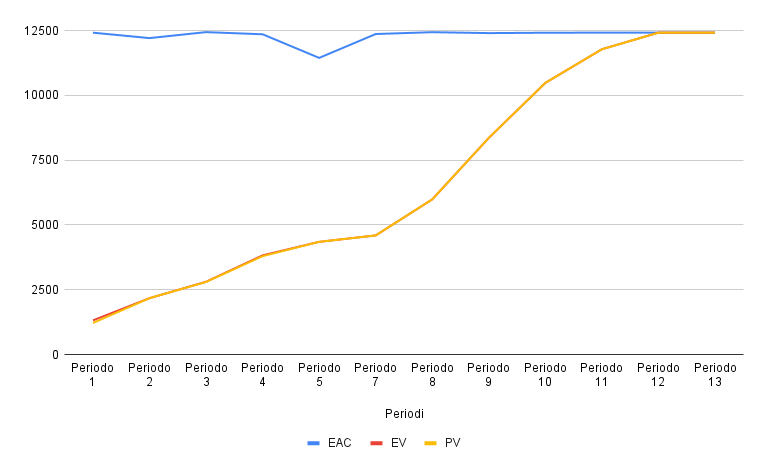
\includegraphics[width=1\textwidth]{../Images/PianoDiQualifica/EV_PV.png}
    \caption{Proiezione dell’EV e del PV nei vari periodi di progetto.}
    \label{fig:3}
\end{figure}

\vspace{0.2cm}

\textbf{RTB}: dall'analisi del grafico, è chiaro che le curve del valore guadagnato (Earned Value) e del valore pianificato (Planned Value) si sovrappongono, suggerendo che il lavoro effettivamente completato corrisponde alla pianificazione. 
Questa coincidenza implica un progresso positivo rispetto alla pianificazione del progetto.

\vspace{0.2cm}
\textbf{PB}:  Dall'analisi del grafico, si evince una congruenza pressoché totale tra le traiettorie del valore guadagnato (EV) e del valore pianficato (PV), a conferma dell'allineamento del completamento del lavoro con la pianificazione originaria.
La convergenza delle due curve con la stima dei costi totali (EAC) nell'ultimo periodo convalida il rispetto del budget preventivato e il completamento dei lavori in linea con le previsioni iniziali.

\subsubsection{M5AC - Actual Cost + M9ETC - Estimate to Complete}

\vspace{0.3cm}

\begin{figure}[H]
    \centering
    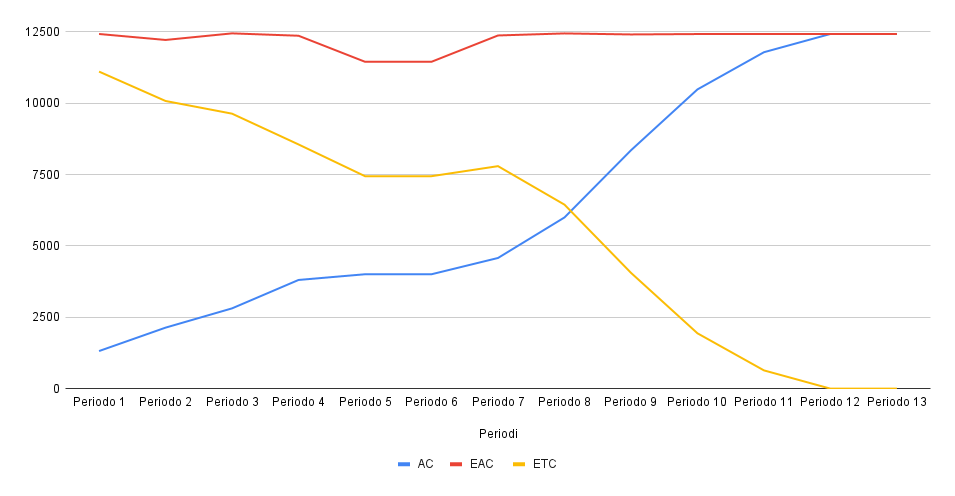
\includegraphics[width=1\textwidth]{../Images/PianoDiQualifica/AC_ETC.png}
    \caption{Proiezione dell’AC e dell’ETC nei vari periodi di progetto.}
    \label{fig:4}
\end{figure}

\vspace{0.2cm}

\textbf{RTB}: il grafico illustra l'Actual Cost (AC), che rappresenta i costi effettivamente sostenuti fino al periodo corrente per il lavoro eseguito, e l'Estimate to Complete (\textit{ETC}\textsubscript{\textit{G}}), che denota la stima dei costi rimanenti per completare il progetto durante i vari periodi.

\vspace{0.2cm}

Si osserva che l'\textit{ETC}\textsubscript{\textit{G}} tende a diminuire, come atteso, mentre l'AC mostra un incremento proporzionale alla riduzione dell'\textit{ETC}\textsubscript{\textit{G}}.

\vspace{0.2cm}
\textbf{PB}: il grafico illustra l'Actual Cost (AC), ossia i costi effettivi sostenuti per il lavoro completato fino al periodo corrente, convergere con l'Estimated at Completion (EAC) nell'ultimo periodo.
Ciò significa che i costi sostenuti sono stati in linea con la stima del costo totale del progetto, a dimostrazione di un efficace controllo e gestione delle risorse finanziarie. Inoltre, l'andamento dell'Estimate to Complete (ETC), ovvero la stima dei costi residui necessari per completare il progetto, evidenzia una graduale diminuzione nel corso del tempo, fino ad azzerarsi nel periodo finale.

\vspace{0.2cm}
Tale risultato conferma il completamento del progetto in linea con le previsioni di budget e la corretta pianificazione delle attività.

\subsubsection{M4BV - Budget Variance + M6SV - Schedule Variance}

\vspace{0.3cm}

\begin{figure}[H]
    \centering
    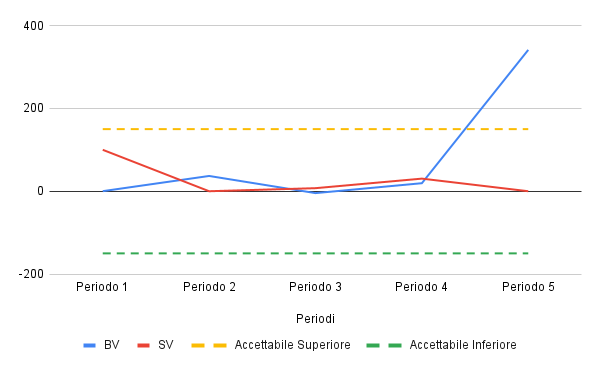
\includegraphics[width=1\textwidth]{../Images/PianoDiQualifica/BV_SV.png}
    \caption{Proiezione della BV e della SV nei vari periodi di progetto.}
    \label{fig:5}
\end{figure}

\vspace{0.2cm}

\textbf{RTB}: il grafico mostra l'andamento della Budget Variance \textit{(BV)} rappresentante la differenza tra il valore guadagnato \textit{(EV)} e i costi sostenuti \textit{(AC)} e la Schedule Variance \textit{(SV)} che indica la differenza tra il valore guadagnato \textit{(EV)} e il valore pianificato (\textit{PV}\textsubscript{\textit{G}}).

\vspace{0.2cm}

Si nota come la Budget Variance risulti altalenante, suggerendo che ad ogni periodo, tranne il primo e il terzo dove abbiamo un valore molto vicino a zero, ci sia una discrepanza dal costo preventivato a quello effettivo fino al periodo di riferimento. 

\vspace{0.2cm}

Nell'ultimo periodo si nota un grande aumento della Budget Variance, questo è dovuto al fatto che le \textit{attività}\textsubscript{\textit{G}} rimanenti sono state completate con un costo inferiore a quello preventivato. 

\vspace{0.2cm}
La Schedule Variance risulta altalenante in alcuni periodi, suggerendo che durante questi intervalli di tempo ci sono stati ritardi o anticipi rispetto alla pianificazione prevista.

\vspace{0.2cm}

Nell'ultimo periodo si è raggiunto l'ottimo per la Schedule Variance. 

\vspace{0.2cm}
\textbf{PB}: Dall'analisi del grafico si nota che la Budget Variance (BV), che rappresenta la differenza tra il valore guadagnato (EV) e i costi sostenuti (AC), si attesta su valori prossimi all'ottimale dopo i periodi relativi all'RTB, indicando un'efficace gestione dei costi e un'accurata stima delle risorse necessarie per il completamento dei lavori.
Analogamente, la Schedule Variance (SV), che indica la differenza tra il valore guadagnato (EV) e il valore pianificato (PV), raggiunge valori ottimali. Questo conferma una pianificazione efficace e un puntuale rispetto dei tempi previsti per il completamento dei lavori.

\subsubsection{M3CPI - Cost Performance Index}

\vspace{0.3cm}

\begin{figure}[H]
    \centering
    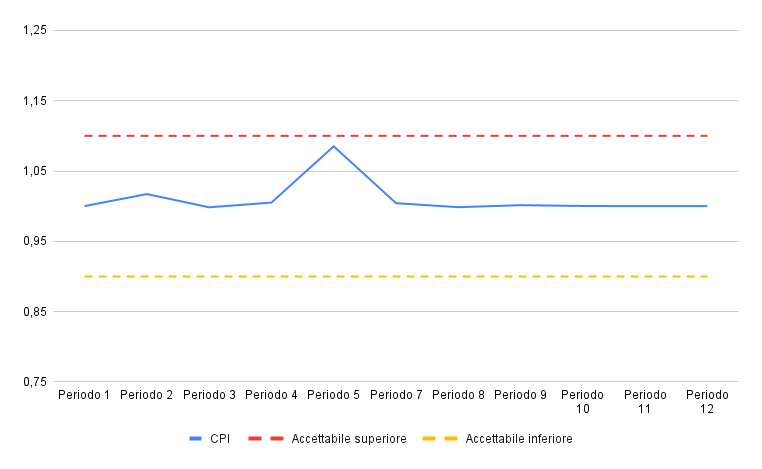
\includegraphics[width=1\textwidth]{../Images/PianoDiQualifica/M3CPI.png}
    \caption{Proiezione del CPI nei vari periodi di progetto.}
    \label{fig:6}
\end{figure}

\vspace{0.2cm}

\textbf{RTB}: il grafico evidenzia la costante prossimità del nostro Cost Performance Index (\textit{CPI}\textsubscript{\textit{G}}) a 1, suggerendo che il progetto stia mantenendo i costi in linea con la pianificazione.

\vspace{0.2cm}

In particolare, nell'ultimo periodo, si osserva un incremento del \textit{CPI}\textsubscript{\textit{G}}, indicando che le \textit{attività}\textsubscript{\textit{G}} rimanenti sono state completate con un costo inferiore rispetto a quanto inizialmente previsto.

\vspace{0.2cm}
\textbf{PB}: il grafico mostra un Cost Performance Index (CPI) costantemente prossimo a 1, a conferma di un'efficace gestione dei costi e di un'accurata stima delle risorse necessarie per il completamento dei lavori.

\subsubsection{M11RNP - Rischi non previsti}

\vspace{0.3cm}

\begin{figure}[H]
    \centering
    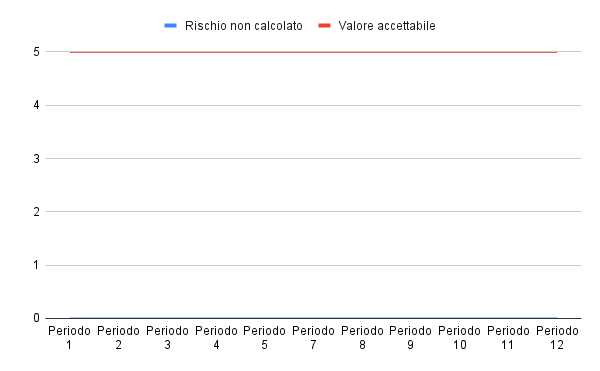
\includegraphics[width=1\textwidth]{../Images/PianoDiQualifica/M11RNP.png}
    \caption{Proiezione rischi non previsti nei vari periodi di progetto.}
    \label{fig:7}
\end{figure}

\vspace{0.2cm}

\textbf{RTB}: il grafico mostra come i rischi non previsti siano rimasti costanti durante tutto il progetto. Questo è un buon segno, in quanto indica che il gruppo è stato in grado di gestire i rischi in modo efficace e che non sono emersi nuovi rischi inaspettati.

\vspace{0.2cm}
\textbf{PB}: Il grafico mostra che, nei periodi successivi, i rischi imprevisti sono rimasti stabili, ad eccezione dell’ultimo periodo. Durante quest’ultimo, si è verificato un rischio non anticipato, che ha causato un incremento minore nei tempi di preparazione per i colloqui previsti per la revisione PB.
